\documentclass[border=10pt]{standalone}
\usepackage{tkz-graph}
\GraphInit[vstyle = Classic]
\tikzset{
  LabelStyle/.style = { rectangle, rounded corners, 
                        fill = white!50,
                        text = black, font = \small\bfseries },
  VertexStyle/.append style = { fill=white,thick, minimum size=25pt,
                                font = \Large\bfseries, thick},
  EdgeStyle/.append style = {-> , font=\bfseries} }
\thispagestyle{empty}
\begin{document}
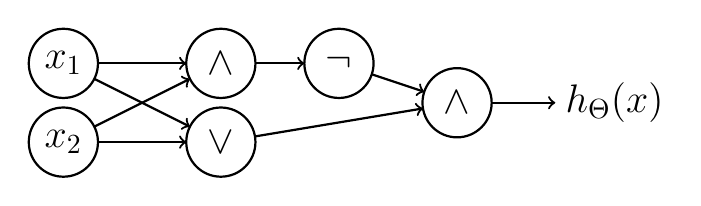
\begin{tikzpicture}
  \SetGraphUnit{45pt}
  \node[VertexStyle](AND1) at (0,0.5) {$\land$}; 
  \node[VertexStyle](OR) at (0,-0.5) {$\lor$}; 
  \node[VertexStyle](X1) at (-2,0.5){$x_1$};
  \node[VertexStyle](X2) at (-2,-0.5){$x_2$};
  \node[VertexStyle](NEG) at (1.5,0.5){$\neg$};
  \node[VertexStyle](AND2) at (3,0){$\land$};
  \node[draw=none, thick, font=\Large\bfseries](END) at (5,0){$h_\Theta(x)$};

  \Edge[](X1)(AND1)
  \Edge[](X2)(AND1)
  \Edge[](X1)(OR)
  \Edge[](X2)(OR)

  \Edge[](AND1)(NEG)
  \Edge[](NEG)(AND2)
  \Edge[](OR)(AND2)
  \Edge[](AND2)(END)
\end{tikzpicture}
\end{document}
